\documentclass[journal,10pt,twocolumn]{article}
\usepackage{graphicx}
\usepackage[margin=0.5in]{geometry}
\usepackage[cmex10]{amsmath}
\usepackage{array}
\usepackage{booktabs}
\usepackage{makecell}
\title{\textbf{Line Assignment}}
\author{Hari Venkateswarlu}
\date{September 2022}
\usepackage[framemethod=tikz]{mdframed}
\newcommand{\myvec}[1]{\ensuremath{\begin{pmatrix}#1\end{pmatrix}}}
\let\vec\mathbf
\newcommand{\mydet}[1]{\ensuremath{\begin{vmatrix}#1\end{vmatrix}}}
\providecommand{\mbf}{\mathbf}
\providecommand{\pr}[1]{\ensuremath{\Pr\left(#1\right)}}
\providecommand{\qfunc}[1]{\ensuremath{Q\left(#1\right)}}
\providecommand{\sbrak}[1]{\ensuremath{{}\left[#1\right]}}
\providecommand{\lsbrak}[1]{\ensuremath{{}\left[#1\right.}}
\providecommand{\rsbrak}[1]{\ensuremath{{}\left.#1\right]}}
\providecommand{\brak}[1]{\ensuremath{\left(#1\right)}}
\providecommand{\lbrak}[1]{\ensuremath{\left(#1\right.}}
\providecommand{\rbrak}[1]{\ensuremath{\left.#1\right)}}
\providecommand{\cbrak}[1]{\ensuremath{\left\{#1\right\}}}
\providecommand{\lcbrak}[1]{\ensuremath{\left\{#1\right.}}
\providecommand{\rcbrak}[1]{\ensuremath{\left.#1\right\}}}

\begin{document}

\maketitle
\paragraph{\textit{Problem Statement} - Find a point on the x-axis,which is equidistant from the points$\begin{pmatrix}
  7 \\
  6 \\
 \end{pmatrix}$ and $\begin{pmatrix}
  3 \\
  4 \\
 \end{pmatrix}$}
\begin{center}
    \label{tab:truthtable}
    \setlength{\arrayrulewidth}{0.2mm}
\setlength{\tabcolsep}{5pt}
\renewcommand{\arraystretch}{1.25}
    \begin{tabular}{|c|c|c|}
    \hline % <-- Alignments: 1st column left, 2nd middle and 3rd right, with vertical lines in between
      \large\textbf{Symbol} & \large\textbf{Co-ordinates} & \large\textbf{Description}\\
      \hline
       \large A1 & $\ \begin{pmatrix} 7\\ 6 \end{pmatrix}$ & co-ordinates of A \\
       \large B1 & $\ \begin{pmatrix} 3\\ 4 \end{pmatrix}$ & co-ordinates of B \\
	
	\large P & $\ \begin{pmatrix} x \\ 0 \end{pmatrix}$ &\makecell {lying on x-axis } \\
      \hline
   \end{tabular}
 \end{center}\vspace{5mm}

\begin{figure}[h]
\centering
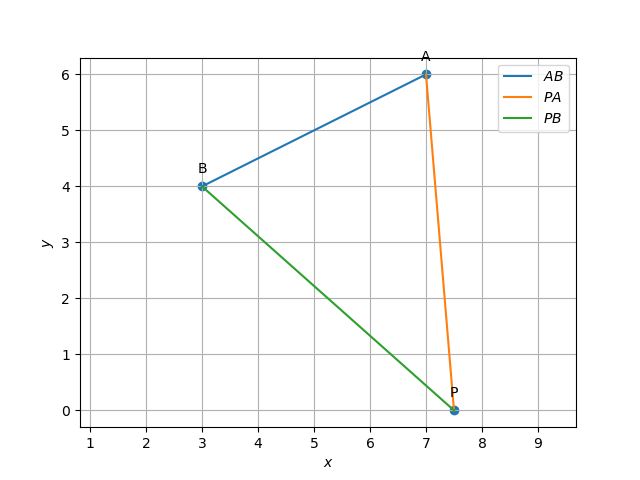
\includegraphics[width=1\columnwidth]{Figure1.png}

\label{fig}
\end{figure}

\section*{Solution}
1. Given points
A=$\begin{pmatrix}
  7 \\
  6 \\
 \end{pmatrix}$
 and B=$\begin{pmatrix}
  3 \\
  4 \\
 \end{pmatrix}$


\raggedright 2. If the point is lying on x-axis then y-axis will be zero i.e.. y=0


\raggedright 3. Distance between the points  $\begin{pmatrix}
  7 \\
  6 \\
 \end{pmatrix}$ and $\begin{pmatrix}
  x \\
  0 \\
 \end{pmatrix}$ is equal to distance between the points $\begin{pmatrix}
  3 \\
  4 \\
 \end{pmatrix}$ and $\begin{pmatrix}
  x \\
  0 \\
 \end{pmatrix}$\\ 	     

\raggedright 4. Consider P on x-axis P$\begin{pmatrix}
  x \\
  0 \\
 \end{pmatrix}$           \vspace{3mm}
\begin{align}
	||\vec{A-P}|| = ||\vec{B-P}||
\end{align}  
    $||\vec{(A-P)}||^2 = \vec{{(A-P)}^{\top}{(A-P)}}$\\
    
$ \vec{\|(A-P)\|}^2 = \myvec{A1\\A2}\myvec{A1 & A2}$ \\
$ \vec{\|(A-P)\|}^2 = (A1)^2+(A2)^2$ \\
    $||\vec{(B-P)}||^2 =  \vec{{(B-P)}^{\top}{(B-P)}}$\\   
    $||\vec{(B-P)}||^2 = \myvec{B1\\B2}\myvec{B1 & B2}$\\
    $||\vec{(B-P)}||^2 = (B1)^2+(B2)^2$ \\
    \vspace{1mm}
 \raggedright 5. From equation 1 
 \\
    \vspace{1mm}            
\begin{gather*}
 (7-x)^2+36=(3-x)^2+16\\                      
 (7-x)^2+20=(3-x)^2\\                         
 49+x^2-14x+20=9+x^2-6x\\                     
 60=8x\\                                    
 x=60/8\\                               
 x=7.5   
\end{gather*}               			
\end{document}
